\subsection{Reparametrization-based Methods}
Research has shown that the intrinsic dimensions of a model reduce when it is fine-tuned for a specific task \cite{aghajanyan2020intrinsic}. Therefore, in theory, a low-dimension reparametrization that is as effective as the full parameter space can be used for fine-tuning \cite{aghajanyan2020intrinsic}.

\subsubsection{LoRA}
LoRA \cite{hu2021lora} uses this information and the hypothesis that the updates made during fine-tuning also have a low intrinsic dimension to create a low-rank weight updating PEFT method. It works on the weight matrices of linear layers by inserting two trainable lower-rank matrices (LoRA weights) that represent the change of the original matrix as seen on \Cref{lora-reparam}.

\begin{figure}[h]
    \centering
    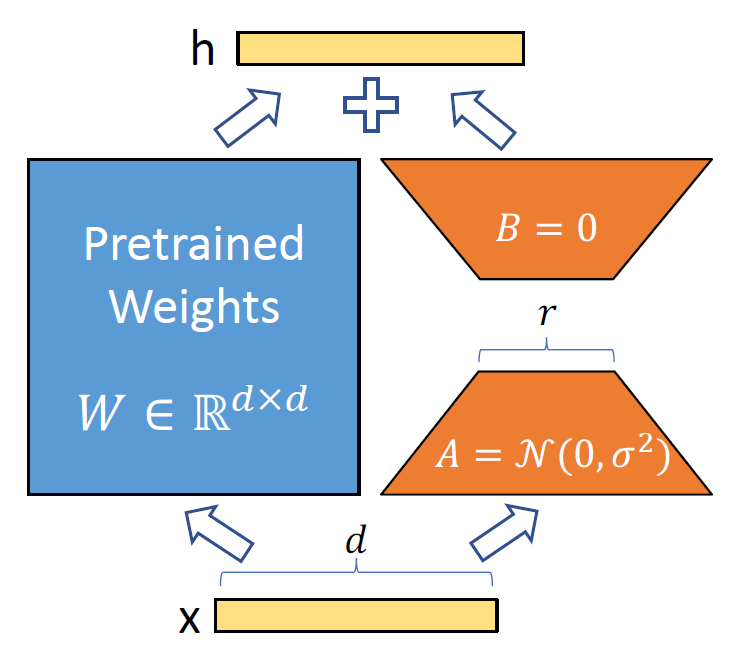
\includegraphics[width=0.6\linewidth]{assets/images/lora-reparametrization.png}
    \caption{The reparametrization of LoRA \cite{hu2021lora}. Only A and B are trained.}
    \label{lora-reparam}
\end{figure}

During training, the pretrained weight matrix (\(W_0\)) of the linear layer is frozen, and the LoRA weights, represented by a down projection (\(A\)) and an up projection (\(B\)) layer, are trained. During the forward pass, the two lower-rank matrices are multiplied together and then added to the original matrix to generate the updated weight matrix for that specific linear layer. For a linear transformation \(h = W_0 x\), the modified forward pass of LoRA yields:

\begin{equation}
    h = W_0 x + B A x
\end{equation}

The down projection layer is randomly initialized, while the up projection layer is initialized to zero. This ensures that their initial multiplication, which represents the change of the weight matrix, is zero. For inference, LoRA weights can be merged with the original weight matrix to get an unmodified model that has the updated weight matrices.

\subsubsection{LoRA-like Models}
Recent advancements in reparametrization-based methods have all used the same approach of freezing the original weight matrix and representing the updates on lower-rank update matrices. These methods include KronA \cite{edalati2022krona}, which uses the Kronecker products of two low-rank matrices to represent the updates; IA\textsuperscript{3} \cite{ia3}, which reimplements the forward pass of LoRA as \(h = (W_0 (x \circ A)) \circ B\) and applies LoRA to only the key and value layers in self-attention and the feed-forward layers in the transformer; and QLoRA \cite{dettmers2023qlora}, which keeps the original weights in a lower-precision data type while applying LoRA. We compare our method directly to LoRA as the other reparametrization-based methods use the same approach and only introduce incremental improvements over LoRA.